
\begin{frame}{Android - Ein Werdegang}
	\begin{itemize}[<+->]
		\item[2003 -] Android, gegründet von Andy Rubin
		\begin{itemize}	
			\item<1-> Unternehmen zur Entwicklung von Mobilsoftware \\(urspr. für Digitalkameras)
		\end{itemize}
		\item[2005 -] Übernahme durch Google
		\item[2007 -] Ankündigung eines neuen Mobiltelefon-OS der Open Handset Alliance
		\item[2008 -] Veröffentlichung des ersten Android OS
		\item[2015 -] Google trennt Sicherheitsupdates von Android-Upgrades
	\end{itemize}
\end{frame}

\begin{frame}{Das Nexus - Der direkte Draht zu Android}
	\begin{itemize}[<+->]
		\item Die Nexus Serie wurde zwischen 2010 und 2016 von Hardwarepartnern hergestellt
		\item Sie erhielt immer die topaktuelle Software aus dem Hause Google
		\item Nexus wurde 2016 durch Pixel abgelöst.
	\end{itemize}
\end{frame}

\begin{frame}{Der Erfolg eines freien Betriebssystems}
	\begin{figure}
		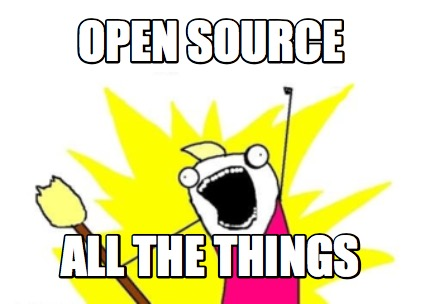
\includegraphics[scale=0.35]{resources/att.jpg}
	\end{figure}
	\begin{itemize}[<+->]
		\item Freiheit des Codes trug zur Fehlersuche und Verbreitung bei
		\item Offener Code ermöglichte Entwicklercommunities wie XDA-Developers
	\end{itemize}
\end{frame}

\begin{frame}{Der Erfolg eines freien Betriebssystems}
	\begin{itemize}[<+->]
		\item Das kostenlosen und freie Android wurde schnell beliebt
		\item 2016 war das OS zu 87,5\% auf dem Markt vertreten
		\item Dabei ist das System stark fragmentiert
		\begin{itemize}
			\item Viele Hersteller verbreiten eigene Portierungen des Systems
			\item Viele CustomROMs von bspw. XDA-Developers fragmentieren zusätzlich 
		\end{itemize}
	\end{itemize}
\end{frame}